\documentclass[12pt]{article}
\usepackage{tcolorbox}% http://ctan.org/pkg/tcolorbox
\definecolor{mycolor}{rgb}{0.122, 0.435, 0.698}% Rule colour
\definecolor{azure}{rgb}{0.94, 1.0, 1.0}
\definecolor{mGreen}{rgb}{0,0.6,0}
\definecolor{mGray}{rgb}{0.5,0.5,0.5}
\definecolor{mPurple}{rgb}{0.58,0,0.82}
\definecolor{backgroundColour}{rgb}{0.95,0.95,0.92}
\usepackage{hyperref}
\usepackage{graphicx}
\usepackage{listings}
\usepackage{float}
\usepackage{textcomp}
\usepackage[normalem]{ulem}
\usepackage{geometry}
\usepackage{xcolor}
 \geometry{
 a4paper,
 total={170mm,235mm},
 left=15mm,
 right=15mm,
 top=25mm,
 }
 
\lstdefinestyle{PyStyle}{
	backgroundcolor=\color{pink},   
	commentstyle=\color{mGreen},
	keywordstyle=\color{magenta},
	numberstyle=\tiny\color{mGray},
	stringstyle=\color{mPurple},
	basicstyle=\footnotesize,
	breakatwhitespace=false,         
	breaklines=true,                 
	captionpos=b,                    
	keepspaces=true,                 
	numbers=left,                    
	numbersep=5pt,                  
	showspaces=false,                
	showstringspaces=false,
	showtabs=false,                  
	tabsize=2,
	language=Python
}
\hypersetup{
	colorlinks=true,
	linkcolor=blue,
	filecolor=magenta,      
	urlcolor=cyan,
}
\urlstyle{same}



\begin{document}

\title{Deep Learning 182, HW \#1}
\author{
Roy Uziel\\
203398854
\and Irit Chelly\\
021565510
}
\date{\today}
\maketitle


\section{Network architecture}
In our graph we used convolutional layers.
The input image is of size 28*28.
\begin{lstlisting}[style=PyStyle]
new_input = tf.reshape(input_images, [-1, 28, 28, 1])   
\end{lstlisting}

We defined the following hidden layers:
\begin{enumerate}

\item
Convolutional Layer 1:\\
We used 32 filters, each filter is a kernel of size 5*5. Each neuron in this layer is a result (scalar) of a convolution of each kernel centered on one neuron in the input layer. Thus, this layer consists of 28*28*32 neurons.
We then compute the activation function relu on the result of each neuron:
\begin{lstlisting}[style=PyStyle]
    conv1 = tf.layers.conv2d(
            inputs=new_input,
            filters=32,
            kernel_size=[5, 5],
            padding="same",
            activation=tf.nn.relu)
\end{lstlisting}

\item
Pooling Layer 1:\\
Here we reduce	 the spatial size of the conv. layer by using a Max Pooling filter of size 2*2 and apply the maximum value of each 2*2 sized part of the image (Convolutional Layer 1). After this step we will have 14*14*32 neurons.: 

\begin{lstlisting}[style=PyStyle]
pool1 = tf.layers.max_pooling2d(inputs=conv1, pool_size=[2, 2], strides=2)
\end{lstlisting}

\item
Convolutional Layer 2:\\
Here we used 64 filters, each filter is a kernel of size 5*5:
\begin{lstlisting}[style=PyStyle]
  conv2 = tf.layers.conv2d(
        inputs=pool1,
        filters=64,
        kernel_size=[5, 5],
        padding="same",
        activation=tf.nn.relu)
\end{lstlisting}

\item
Pooling Layer 2:\\
After this step we will have 7*7*64 neurons:
\begin{lstlisting}[style=PyStyle]
      pool2 = tf.layers.max_pooling2d(inputs=conv2, pool_size=[2, 2], strides=2)
\end{lstlisting}

\item
Reshaping:
\begin{lstlisting}[style=PyStyle]
         pool2_flat = tf.reshape(pool2, [-1, 7 * 7 * 64])
\end{lstlisting}

\item
Dense:\\
This layer is fully connected: we picked 1024 neurons in this layer that are fully connected to the neurons from the previous layer ("Pooling Layer 2"):
\begin{lstlisting}[style=PyStyle]
         dense = tf.layers.dense(inputs=pool2_flat, units=1024, activation=tf.nn.relu)    
\end{lstlisting}

\item
Dropout:
\begin{lstlisting}[style=PyStyle]
    dropout = tf.layers.dropout(inputs=dense, rate=0.2)
\end{lstlisting}

\item
Output:\\
The output layer is 10 neurons, each neuron is a classifier for one digit. This layer is full connected to the previous layer:
\begin{lstlisting}[style=PyStyle]
    logits = tf.layers.dense(inputs=dropout, units=10)
\end{lstlisting}

\end{enumerate}

\begin{figure}[H]
\caption{Architecture Description Graph}
\centering
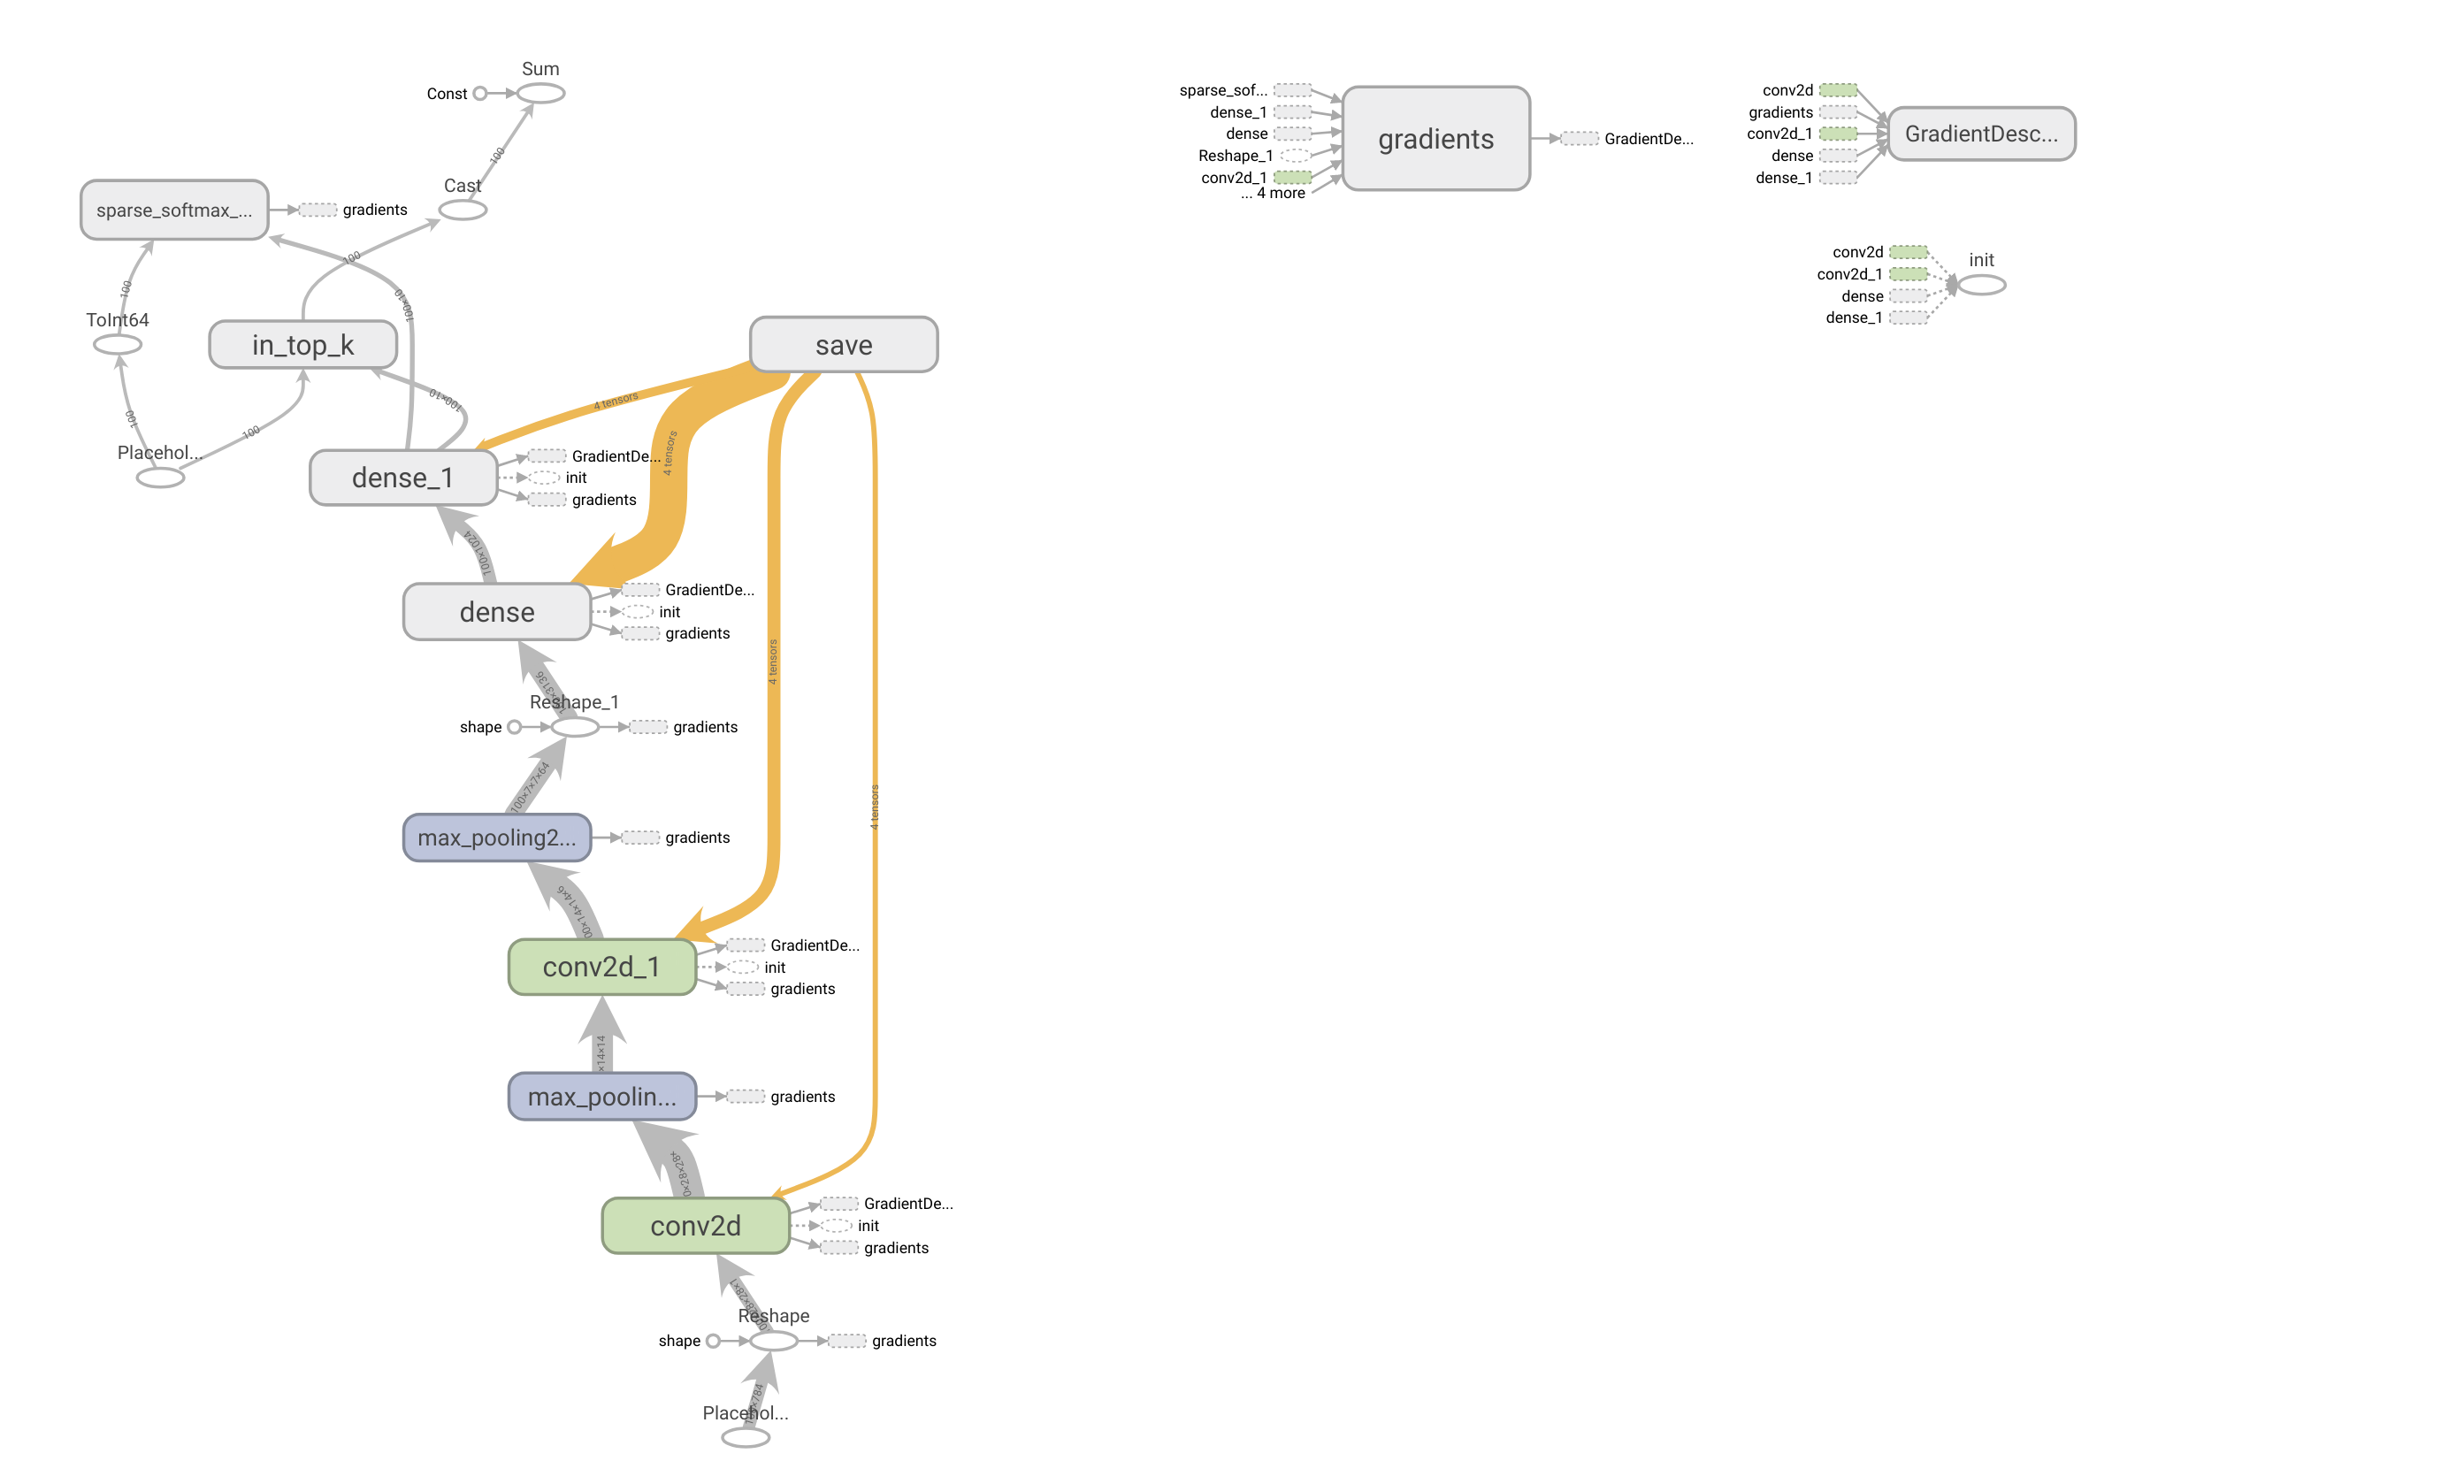
\includegraphics[width=\linewidth]{Graphs.png}
\end{figure}

\newpage

\section{Results}

Below are the script results after running with 100 batches and 4000 steps to run the trainer, reaching precision of $0.97$:\\

Training Data Eval:\\
Num examples: 55000  Num correct: 53798  Precision @ 1: 0.9781\\
Validation Data Eval:\\
Num examples: 5000  Num correct: 4896  Precision @ 1: 0.9792\\
Test Data Eval:\\
Num examples: 10000  Num correct: 9778  Precision @ 1: 0.9778\\
An exception has occurred, use \\

\begin{figure}[H]
\caption{Loss Function Graph}
\centering
  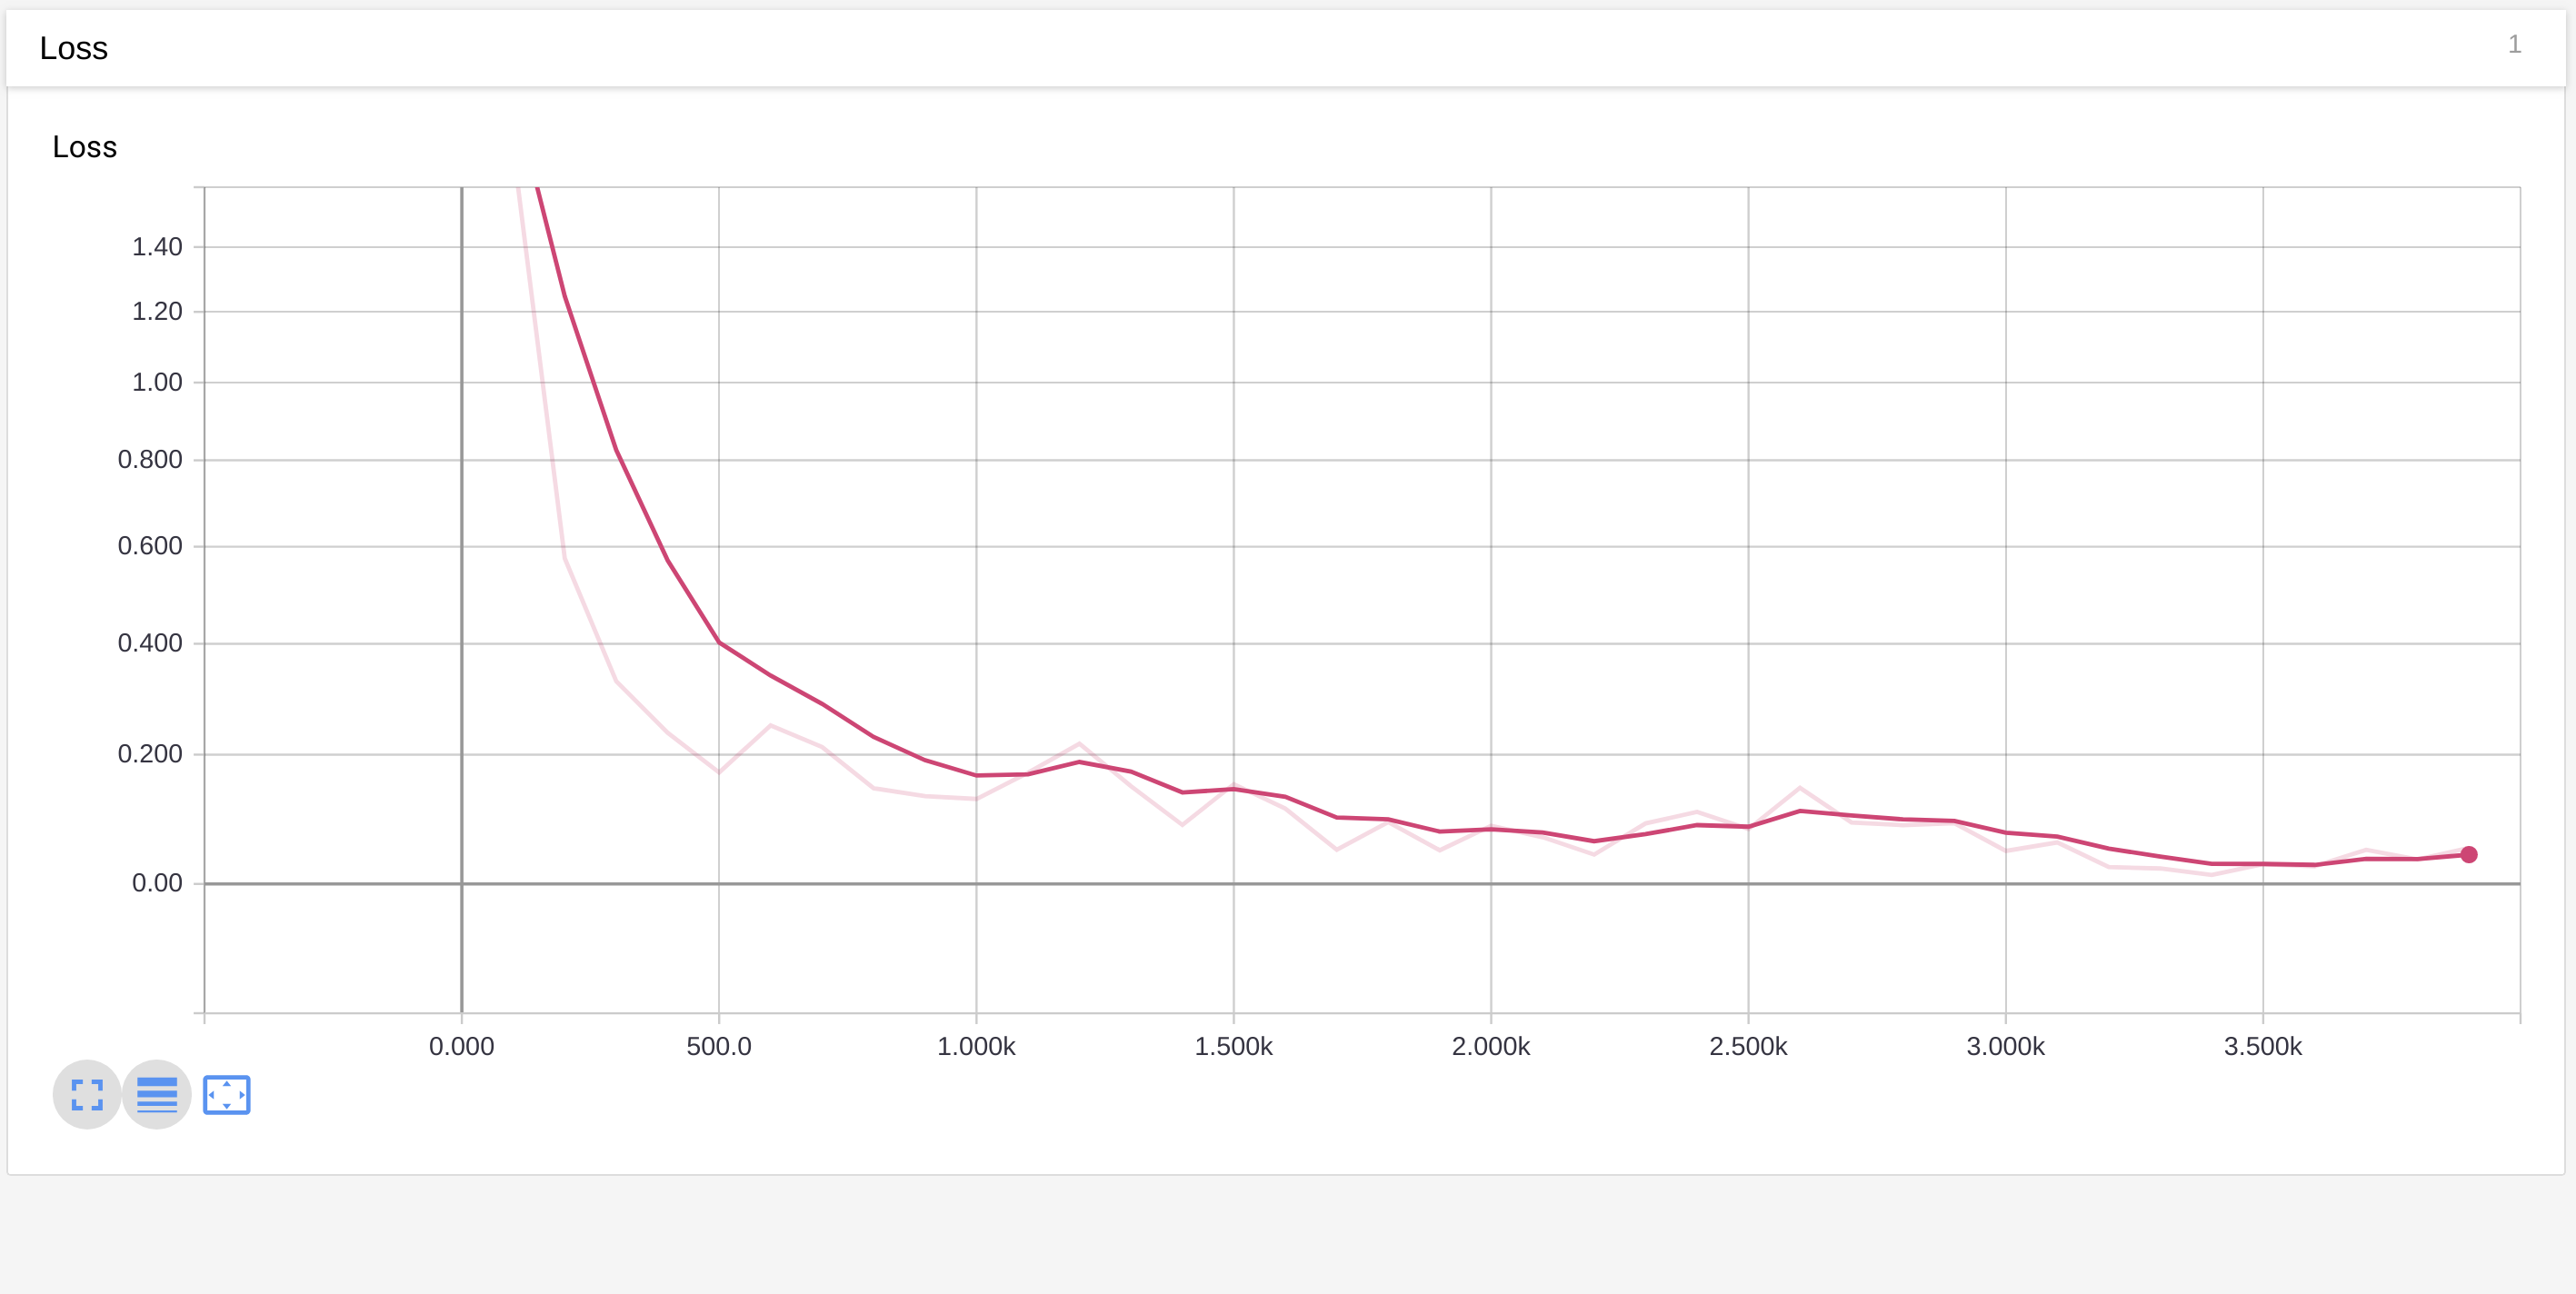
\includegraphics[width=\linewidth]{Loss.png}
\end{figure}


\begin{figure}[H]
\caption{Console results and parameters:}
\centering
  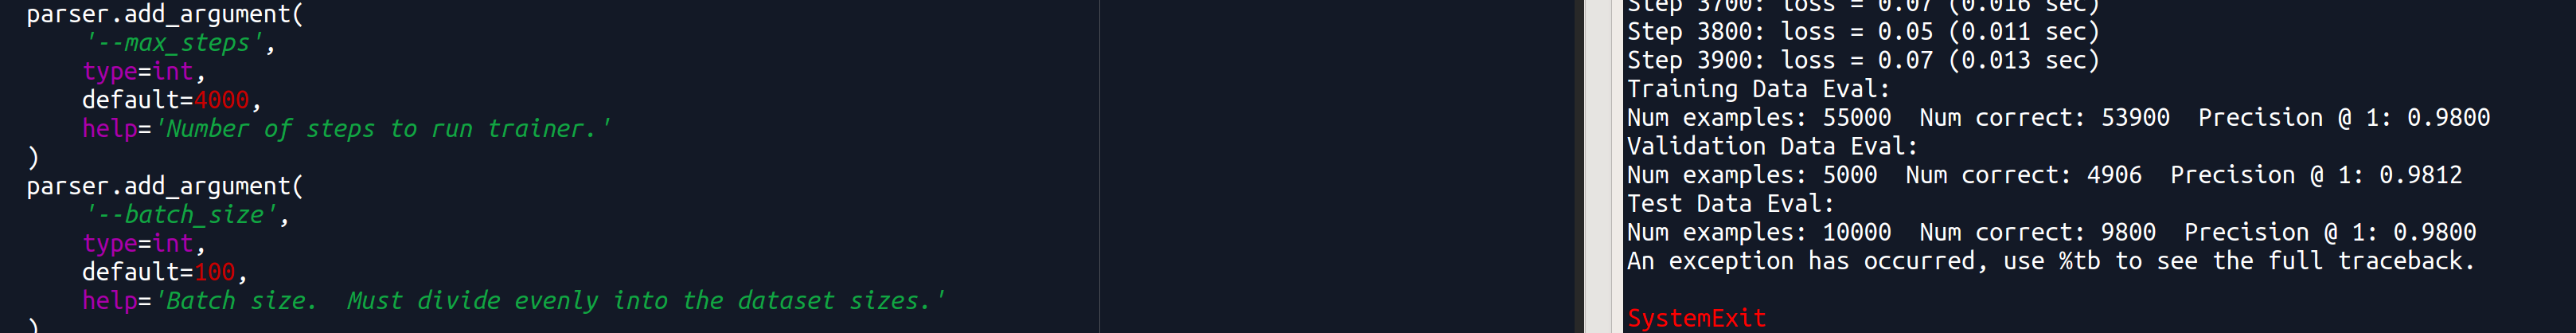
\includegraphics[width=\linewidth]{spyder-console.png}
\end{figure}


\end{document}